Few algorithms are better known than Dijkstra's Algorithm~\cite{dijkstra:note:1959} amongst working Computer Scientists, belying the importance of shortest path algorithms to the field.
Most textbook presentations of Dijkstra's Algorithm (see, for example,~\cite[Chapter 24]{clrs}) are particularly concrete, presenting the algorithm as working over directed graphs with non-negative numeric arc weights.
Interestingly, but potentially less well known, the algorithm exists in a more general form where path weights are not numeric but drawn from a large class of \emph{semirings}~\cite{gondran_graphs_2008, mohri:semiring:2002}.

Recall that a semiring $\langle S, \oplus, \otimes, 0, 1 \rangle$ is composed of a commutative monoid $\langle S, \oplus, 0\rangle$ and a monoid $\langle S, \otimes, 1\rangle$ such that two \emph{distributivity} and an \emph{annihilation} axiom hold, connecting the two substructures:
\begin{gather*}
a\otimes (b \oplus c) = (a\otimes b) \oplus (a\otimes c) \qquad
(b \oplus c) \otimes a = (b\otimes a) \oplus (c\otimes a) \qquad
0 \otimes a = 0
\end{gather*}
Now, given an adjacency matrix over a semiring, $\mathbf{A}$, representing a weighted, directed graph, the generalised shortest-path problem is the task of finding a matrix $\mathbf{A}^*$ such that
\begin{gather*}
\label{eq:global}
\mathbf{A}^*(i,\ j) = \displaystyle\bigoplus_{p \in \mathcal{P}(i,\ j)} w_{\mathbf{A}}(p)
\end{gather*}
where $\mathcal{P}(i,\ j)$ represents the set of all paths from node $i$ to node $j$ and $w_{\mathbf{A}}(p)$ is the \emph{weight} of a path.
Given a path $p = v_0, v_1, \ldots, v_k$---a sequence of nodes---this is defined as
\begin{gather*}
    w_{\mathbf{A}}(p)
    \equiv
    \mathbf{A}(v_0,\ v_1)
    \otimes \mathbf{A}(v_1,\ v_2)
    \otimes \cdots
    \otimes \mathbf{A}(v_{k-1},\ v_k),
\end{gather*}
with the empty path assigned the weight $1$.
The matrix $\mathbf{A}^*$ need not always exist, but it is well known that if it does then it is a solution for $\mathbf{R}$ in the following right equation
\begin{gather*}
\mathbf{R} = (\mathbf{R} \otimes \mathbf{A}) \oplus \mathbf{I}
\end{gather*}
where $\mathbf{I}$ is the identity matrix, and the multiplication and addition operations of the semiring have been lifted to matrix multiplication and addition in the `obvious' manner, with solutions to these equations encoding the path weights of shortest paths between nodes of the graph.
Single source shortest path algorithms, such as Dijkstra's Algorithm, may then be seen as computing one row of a solution to the above fixpoint equation.

A nice feature of working in this algebraic setting is that the semiring parameterising the algorithm can be varied: some semirings cause the algorithm to compute shortest paths through the graph, \emph{a la} traditional presentations of Dijkstra, whereas other cause the algorithm to compute maximum bottleneck capacity, or some other feature of the graph.
The key idea here is that a generic, parametric implementation of a shortest path algorithm can be developed and then instantiated with different semirings, and thereafter uniformly used to calculate different properties of graphs.
The interested reader can find a thorough treatment of this material in~\cite{gondran_graphs_2008}.

Further, we may ask what happens when we vary the underlying algebraic structure, for example by weakening the axioms of a semiring.
In particular, it can be seen that Dijkstra's Algorithm relies crucially on the distributivity axioms of the underlying semiring to compute \emph{globally optimal} paths.
However, recent work on mathematically modelling the Border Gateway Protocol (BGP), the Internet routing protocol which maintains connectivity between Internet Service Providers, has led to the idea of \emph{local} optimal paths (also called equilibrium solutions). where the underlying algebraic structure, in contrast to semirings, is non-distributive~\cite{sobrinho_routing_2010}.
In this relaxed, non-distributive setting, Dijkstra's Algorithm once more computes solutions to the right fixed-point equation above, but these solutions are now locally optimal, rather than global.

In this paper, we present an implementation of a generalised, non-distributive variant of Dijkstra's Algorithm.
In order to 
Our algorithm is a variant of Dijkstra's algorithm in the sense that it keeps a queue of all the nodes that have not yet been visited, sorted by their estimated distance from the source node such that the head of the queue is always the unvisited node with the minimum distance estimate. However, unlike the usual description of Dijkstra's algorithm, our implementation is not imperative and sacrifices efficiency for readability.

The correctness proof shows that the algorithm we have implemented does indeed compute the right-local solution given any adjacency matrix representing a graph over the algebra we describe.

%The generalised shortest-path problem is then to find a matrix $\mathbf{A}^*$ such that
%\begin{gather*}
%\label{eq:global}
%\mathbf{A}^*(i,\ j) = \displaystyle\bigoplus_{p \in \mathcal{P}(i,\ j)} w_{\mathbf{A}}(p)
%\end{gather*}
%where $\mathcal{P}(i,\ j)$ represents the set of all paths from node $i$ to node $j$.
%The matrix $\mathbf{A}^*$ need not always exist, but it is well known that if it does then it is a solution for $\mathbf{L}$ or $\mathbf{R}$ in the following left and right equations
%\begin{gather*}
%\mathbf{L} = (\mathbf{A} \otimes \mathbf{L}) \oplus \mathbf{I} \qquad\qquad
%\mathbf{R} = (\mathbf{R} \otimes \mathbf{A}) \oplus \mathbf{I}
%\end{gather*}

% A nice feature of working in this algebraic setting is that the semiring parameterising the algorithm can be varied: some semirings cause the algorithm to compute shortest paths through the graph, \emph{a la} traditional presentations of Dijkstra, whereas other cause the algorithm to compute maximum bottleneck capacity, or some other feature of the graph.
% The key idea here is that a generic, parametric implementation of a shortest path algorithm can be developed and then instantiated with different semirings, and thereafter uniformly used to calculate different properties of graphs.
% The interested reader can find a thorough treatment of this material in~\cite{gondran_graphs_2008}.
%
% The distributivity axioms,
% Equations~\ref{eq:left:distributivity} and~\ref{eq:right:distributivity},
% are essential in the semiring theory outlined above.
% Thus it may seem suprising that recent research has shown that
% the matrix equations ~\ref{eq:left:local} and ~\ref{eq:right:local}
% can sometimes be solved even when
% distributivity axioms do not hold in the algebraic structure employed.
% Much of this work was originally motivated
% by investigations of the Border Gateway Protocol (BGP),
% the Internet routing protocol which has evolved to
% maintain global connectivity between Internet Service Providers (ISPs).
% In BGP the anologue of the weight of a path
% $p = v_0, v_1, \cdots,\ v_k$ at node $v_0$
% is dominated by the contractual relationships between
% the networks associated with nodes $v_0$ and $v_1$.
% The typical relationships involve those between customers
% and providers and between competing ISPs (that must exchange
% routing information in order to provide connectivity to
% the global Internet).
%
% But how can we interpret such solutions?
% Take Equation~\ref{eq:left:local} for example.
% If we assume that $\mathbf{L}$ solves this equation
% and that $i \neq j$, then we have
% \begin{equation}
% \label{eq:left:local:at:i}
% \mathbf{L}(i,\ j) = \displaystyle\bigoplus_{q \in N(i)} \mathbf{A}(i,\ q) \otimes \mathbf{L}(q,\ j),
% \end{equation}
% where $N(i)$ is the set of neighbors of node $i$.
% We can interpret this from node $i$'s perspective as
% the best path weight available given the paths its neighbors
% have obtained.
% That is, $\mathbf{L}$ does not represent the globally optimal
% path weights, but rather an equilibrium point that we will
% call \emph{locally optimal}.
%
% \begin{figure}[ht]
% 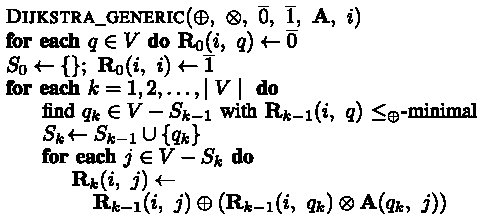
\includegraphics{algorithm.pdf}
% \caption{Dynerowicz and Griffin's imperative generalized Dijkstra's algorithm}
% \label{fig.algorithm}
% \end{figure}

%\todo{finish me}

%Following Sobrinho and Griffin, we call solutions for \(\mathbf{L}\) and \(\mathbf{R}\) \emph{left-local} and \emph{right-local} solutions, respectively; they represent two types of \emph{routing in equilibrium}~\cite{sobrinho_routing_2010}. Their key insight was that a generalized variant of Dijkstra's algorithm finds right-local solutions and a generalized variant of Bellman-Ford gives left-local solutions, both forms of \emph{local optima}, when distributivity does not hold.

\paragraph{Agda}

Agda~\cite{norell_dependently_2009} is a dependently-typed programming language \emph{cum} proof assistant for higher-order intuitionistic logic.
In contrast to similar systems~\cite{bertot_short_2008,asperti_matita_2011} proof terms are constructed by hand via a type-direct refinement process.

Agda has a uniform syntax, though one syntactic novelty is a flexible system of user-declared Unicode mixfix identifiers~\cite{danielsson_parsing_2011} with `holes' in an identifier being denoted by underscores.
We write \AgdaSymbol{(}\AgdaBound{x}~\AgdaSymbol{:}~\AgdaBound{A}\AgdaSymbol{)}~\AgdaSymbol{→}~\AgdaBound{B} for the dependent function space where \AgdaBound{x} may occur in \AgdaBound{B}, write \AgdaBound{A}~\AgdaSymbol{→}~\AgdaBound{B} when \AgdaBound{x} does not occur in \AgdaBound{B}, and write \AgdaSymbol{\{}\AgdaBound{x}~\AgdaSymbol{:}~\AgdaBound{A}\AgdaSymbol{\}}~\AgdaSymbol{→}~\AgdaBound{B} (sometimes making use of the shorthands \AgdaSymbol{∀}~\AgdaBound{x}~\AgdaSymbol{→}~\AgdaBound{B} and \AgdaSymbol{∀}~\AgdaSymbol{\{}\AgdaBound{x}\AgdaSymbol{\}}~\AgdaSymbol{→}~\AgdaBound{B}), when types can be inferred.
We write \AgdaDatatype{Σ}~\AgdaBound{A}~\AgdaBound{B} for the dependent sum type whose first projection has type \AgdaBound{A}, and write \AgdaBound{A}~\AgdaDatatype{×}~\AgdaBound{B} when the second projection does not depend on the first, and write \AgdaFunction{∃}~\AgdaSymbol{λ}~\AgdaBound{x}~\AgdaSymbol{→}~\AgdaBound{P} for the dependent sum type when the type of the first projection can be inferred.
Dependent sums are constructed using the comma constructor: \AgdaBound{x}~\AgdaInductiveConstructor{,}~\AgdaBound{y}.
Propositional equality between two types is written \AgdaBound{A}~\AgdaDatatype{≡}~\AgdaBound{B} and has a single canonical inhabitant, \AgdaInductiveConstructor{refl}.
Lastly, we write \AgdaBound{A}~\AgdaDatatype{⊎}~\AgdaBound{B} for disjoint union, with constructors \AgdaInductiveConstructor{inj₁} and \AgdaInductiveConstructor{inj₂}, and \AgdaFunction{¬}~\AgdaBound{A} for negation.

%\paragraph{Contributions and map of paper}
%\subsection{Map of Paper}
%\label{subsect.map.of.paper}
%In Section~\ref{sect.basic.definitions} we cover some definitions needed to define Dijkstra's algorithm and its correctness proof.
%In Section~\ref{sect.path.algebras.their.properties.and.models} we discuss `path algebras', a variety of algebraic structure central to our proof of correctness, also providing three models of path algebras to demonstrate that models exist and that path algebras are not categorical.
%In Section~\ref{sect.dijkstras.algorithm.and.its.correctness} we discuss the imperative Dijkstra algorithm, our functional implementation, and main body of the correctness proof leading up to our main theorem: Dijkstra's algorithm computes a right-local solution.
%In Section~\ref{sect.example} we demonstrate the algorithm in action with an example execution inside Agda.
%In Section~\ref{sect.conclusions} we conclude.
